\documentclass{standalone}
\usepackage{tikz}

\usetikzlibrary{graphs,quotes}
\tikzstyle{block} = [draw, rectangle]
\tikzstyle{sum} = [draw, fill=blue!20, circle, node distance=1cm]
\tikzstyle{input} = [coordinate]
\tikzstyle{output} = [coordinate]
\tikzstyle{pinstyle} = [pin edge={to-,thin,black}]

\begin{document}
% \tikz\graph[grow down=3em]
% {
%   x [as=$\mathbf{x}$]
%   ->[thick] wl1 [block,as=weight layer]
%   ->[thick,"relu"] wl2 [block,as=weight layer]
%   ->[thick] plus [as=$\bigoplus$]
%   ->[thick,"relu"]
%   empty [as=];
%   x ->[thick,bend left=90,distance=5em,"$\mathbf{x}$"] plus;
% };

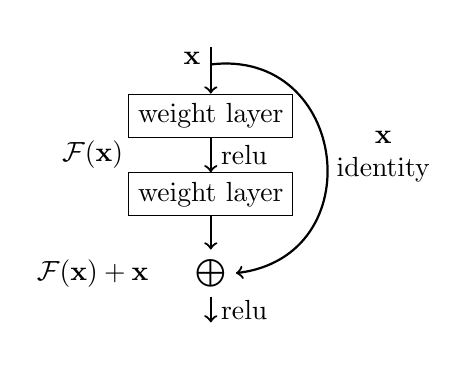
\begin{tikzpicture}
  \node (start) at (0,0) {};
  \node[draw] (wl1) at (0,-1) {weight layer};
  \node[draw] (wl2) at (0,-2) {weight layer};
  \node (plus) at (0,-3) {$\bigoplus$};
  \node (end) at (0,-3.75) {};

  \node (fx) at (-1.5, -1.5) {$\mathcal{F}(\mathbf{x})$};
  \node (fxx) at (-1.5, -3) {$\mathcal{F}(\mathbf{x}) + \mathbf{x}$};

  \draw[->,thick] (start) to node[near start,left] {$\mathbf{x}$} (wl1); 
  \draw[->,thick] (wl1) to node[right] {relu} (wl2); 
  \draw[->,thick] (wl2) to (plus); 
  \draw[->,thick] (plus) to node[right] {relu} (end); 
  \draw[->,thick] (0,-0.35) to[bend left=90,distance=5em] node[right,align=center] {$\mathbf{x}$\\identity} (plus); 
\end{tikzpicture}
\end{document}
%%% Local Variables:
%%% mode: latex
%%% TeX-master: t
%%% End:
